\documentclass[11pt]{article}
\usepackage{amsmath} % For math symbols
\usepackage{amssymb} % For checkmark and other symbols
\usepackage{array} % For better tables
\usepackage{booktabs} % For professional-looking tables
\usepackage{graphicx}

\title{COMS 4733 Homework 2}
\author{Jaisel Singh}
\date{\today}
\begin{document}
\maketitle
\section{Problem 1: Discrete Search Algorithms}
\subsection{Search Algorithm Comparison}
% Define notation
\noindent\textbf{Notation:}
\begin{itemize}
\item $b$ = branching factor (average number of successors per node)
\item $d$ = depth of the shallowest goal node
\item $m$ = maximum depth of the search tree
\end{itemize}
\noindent\textit{Note: All algorithms use graph search (visited set) on finite state space.}

\begin{table}[h]
\centering
\begin{tabular}{|l|c|c|c|c|}
\hline
\textbf{Algorithm} & \textbf{Complete?} & \textbf{Cost-Optimal?} & \textbf{Time Complexity} & \textbf{Space Complexity} \\
\hline
DFS & Yes & No & $O(b^m)$ & $O(bm)$ \\
\hline
BFS & Yes & No & $O(b^d)$ & $O(b^d)$ \\
\hline
Dijkstra & Yes & Yes & $O(b^d)$ & $O(b^d)$ \\
\hline
A* (admissible $h$) & Yes & Yes & $O(b^d)$ & $O(b^d)$ \\
\hline
\end{tabular}
\caption{Comparison of search algorithms}
\label{tab:search_comparison}
\end{table}

\subsubsection{Justification for Selected Entries}

\textbf{Dijkstra's Algorithm - Time Complexity: $O(b^d)$}

Dijkstra's algorithm explores nodes in order of increasing cost from the start node. In the worst case, it must explore all nodes up to the depth $d$ of the optimal solution before guaranteeing it has found the cheapest path.

Consider a tree structure where:
\begin{itemize}
\item At depth 0: 1 node (start)
\item At depth 1: $b$ nodes
\item At depth 2: $b^2$ nodes
\item $\vdots$
\item At depth $d$: $b^d$ nodes
\end{itemize}

The total number of nodes explored is:
$$1 + b + b^2 + \cdots + b^d = \frac{b^{d+1} - 1}{b - 1} = O(b^d)$$

Each node is processed once (removed from the priority queue), and for each of its neighbors, we may perform a priority queue operation. With an efficient priority queue implementation (binary heap), these operations take $O(\log n)$ time where $n$ is the number of nodes in the queue.

Therefore, the overall time complexity is $O(b^d)$ in the context of search algorithms.

\textbf{Dijkstra's Algorithm - Space Complexity: $O(b^d)$}

Dijkstra's algorithm uses a priority queue to store nodes that have been discovered but not yet fully explored. In the worst case, before reaching the goal at depth $d$, the priority queue may contain all nodes at the frontier of the search.

Since Dijkstra's explores in a breadth-first manner (ordered by cost rather than depth), it must maintain all nodes at the current cost level. In a tree with branching factor $b$ and goal at depth $d$, the maximum number of nodes in the priority queue at once is proportional to $b^d$ (the number of nodes at depth $d$).

Additionally, with graph search (using a visited set to avoid cycles), we must store all visited nodes, which is also $O(b^d)$ in the worst case.

Therefore, the space complexity is $O(b^d)$.

\subsection{Search Tree Expansion}

\subsubsection{Task 1: BFS Expansion Order}

Using lexicographic ordering (smallest $x$ first, then smallest $y$) for tie-breaking, the BFS expansion order is:

\begin{center}
\begin{tabular}{|c|c|c|c|}
\hline
\textbf{(0,3)} & \textbf{(1,3)} & \textbf{(2,3)} & \textbf{G (3,3)} \\
5 & 8 & 12 & 14 \\
\hline
\textbf{(0,2)} & \textbf{X (1,2)} & \textbf{(2,2)} & \textbf{(3,2)} \\
2 & - & 9 & 13 \\
\hline
\textbf{S (0,1)} & \textbf{(1,1)} & \textbf{(2,1)} & \textbf{(3,1)} \\
0 & 3 & 6 & 10 \\
\hline
\textbf{(0,0)} & \textbf{(1,0)} & \textbf{(2,0)} & \textbf{(3,0)} \\
1 & 4 & 7 & 11 \\
\hline
\end{tabular}
\end{center}

\textbf{Complete expansion sequence:}
\begin{align*}
&0: S(0,1) \rightarrow 1: (0,0) \rightarrow 2: (0,2) \rightarrow 3: (1,1) \rightarrow 4: (1,0) \rightarrow 5: (0,3) \rightarrow 6: (2,1) \\
&\rightarrow 7: (2,0) \rightarrow 8: (1,3) \rightarrow 9: (2,2) \rightarrow 10: (3,1) \rightarrow 11: (3,0) \rightarrow 12: (2,3) \\
&\rightarrow 13: (3,2) \rightarrow 14: G(3,3)
\end{align*}

\subsubsection{Task 2: Dijkstra's Algorithm}

Dijkstra's algorithm expands nodes in the \textbf{same order} as BFS for this problem.

\textbf{Explanation:} 

BFS and Dijkstra's expand nodes identically because all edges have uniform cost (cost = 1). Dijkstra's algorithm uses a priority queue to explore nodes in order of increasing cumulative cost from the start. Since each move costs 1, a node at distance $d$ from the start has total cost $d$. This matches BFS exactly, which explores nodes layer-by-layer by distance.

When multiple nodes have the same priority (same cost in Dijkstra's, same depth in BFS), both algorithms apply the lexicographic tie-breaking rule. Since cost equals depth in this uniform-cost scenario, both algorithms break ties identically and produce the same expansion order.

Therefore, Dijkstra's expansion order is identical to the BFS grid shown above.

\subsubsection{Task 3: A* with Manhattan Distance Heuristic}

Using the Manhattan distance heuristic $h(x,y) = |3-x| + |3-y|$ and lexicographic tie-breaking, A* expands nodes in the following order:

\begin{center}
\begin{tabular}{|c|c|c|c|c|}
\hline
\textbf{Order} & \textbf{Node} & \textbf{$g(n)$} & \textbf{$h(n)$} & \textbf{$f(n) = g(n) + h(n)$} \\
\hline
0 & S (0,1) & 0 & 5 & 5 \\
\hline
1 & (0,2) & 1 & 4 & 5 \\
\hline
2 & (0,3) & 2 & 3 & 5 \\
\hline
3 & (1,1) & 1 & 4 & 5 \\
\hline
4 & (1,3) & 3 & 2 & 5 \\
\hline
5 & (2,1) & 2 & 3 & 5 \\
\hline
6 & (2,2) & 3 & 2 & 5 \\
\hline
7 & (2,3) & 4 & 1 & 5 \\
\hline
8 & (3,1) & 3 & 2 & 5 \\
\hline
9 & (3,2) & 4 & 1 & 5 \\
\hline
10 & G (3,3) & 5 & 0 & 5 \\
\hline
\end{tabular}
\end{center}

\textbf{Grid with expansion order:}

\begin{center}
\begin{tabular}{|c|c|c|c|}
\hline
\textbf{(0,3)} & \textbf{(1,3)} & \textbf{(2,3)} & \textbf{G (3,3)} \\
2 & 4 & 7 & 10 \\
\hline
\textbf{(0,2)} & \textbf{X (1,2)} & \textbf{(2,2)} & \textbf{(3,2)} \\
1 & - & 6 & 9 \\
\hline
\textbf{S (0,1)} & \textbf{(1,1)} & \textbf{(2,1)} & \textbf{(3,1)} \\
0 & 3 & 5 & 8 \\
\hline
\textbf{(0,0)} & \textbf{(1,0)} & \textbf{(2,0)} & \textbf{(3,0)} \\
- & - & - & - \\
\hline
\end{tabular}
\end{center}

\textbf{Observations/Notes}

\begin{itemize}
    \item All expanded nodes have $f(n) = 5$, which equals the optimal path cost
    \item Nodes in row $y=0$ (bottom row) such as (0,0), (1,0), (2,0), and (3,0) are generated but never expanded because they all have $f = 7 > 5$
    \item The Manhattan distance heuristic is admissible (never overestimates) and consistent in this 4-connected grid with unit costs
    \item Because $h$ is admissible and the grid uses 4-connected movement with unit costs, every node on an optimal path satisfies $g + h = 5$ (constant). Therefore, the expansion order among these nodes is determined purely by the lexicographic tie-breaking rule
    \item A* reaches the goal at step 10, having expanded only 11 nodes (including the start), compared to 15 nodes for BFS
\end{itemize}

\subsection{Heuristic Admissibility}

\subsubsection{Is Euclidean distance admissible?}

\textbf{Answer:} Yes, the Euclidean distance heuristic $h(n) = \sqrt{(x_g - x)^2 + (y_g - y)^2}$ is admissible for this cost model.

\textbf{Justification:}

A heuristic is admissible if it never overestimates the true optimal cost to reach the goal. The Euclidean distance represents the straight-line distance between two points, which is the shortest possible distance in Euclidean space.

With 8-connected movement where diagonal moves cost $\sqrt{2}$ and cardinal moves cost 1, we can analyze the relationship between the heuristic and actual cost:

\begin{itemize}
    \item Consider moving from $(0,0)$ to $(3,3)$:
    \begin{itemize}
        \item Euclidean distance: $h = \sqrt{(3-0)^2 + (3-0)^2} = \sqrt{18} = 3\sqrt{2} \approx 4.243$
        \item Optimal path: Three diagonal moves $(0,0) \rightarrow (1,1) \rightarrow (2,2) \rightarrow (3,3)$
        \item Actual cost: $3\sqrt{2} \approx 4.243$
    \end{itemize}
    \item In general, for any two points, the Euclidean distance equals the cost of moving in a straight diagonal line (when possible), which is the optimal path in an obstacle-free 8-connected grid
    \item Since we cannot move "more directly" than the straight line, and diagonal moves have cost exactly $\sqrt{2}$, the Euclidean distance never overestimates the true cost
\end{itemize}

Therefore, the Euclidean distance heuristic is admissible for this cost model.

\subsubsection{Propose a different admissible heuristic}

\textbf{Answer:} The Chebyshev distance (L$^\infty$ norm) is an admissible heuristic for this cost model:
$$h(n) = \max(|x_g - x|, |y_g - y|)$$

\textbf{Justification:}

The Chebyshev distance measures the maximum absolute difference in either coordinate, which corresponds to the minimum number of moves required to reach the goal when diagonal moves are allowed.

To show admissibility, we verify that this heuristic never overestimates:

\begin{itemize}
    \item The Chebyshev distance counts the number of diagonal or cardinal moves needed along the longer dimension
    \item Example: From $(0,0)$ to $(3,3)$:
    \begin{itemize}
        \item Chebyshev distance: $h = \max(|3-0|, |3-0|) = 3$
        \item Optimal path: Three diagonal moves with cost $3\sqrt{2} \approx 4.24$
        \item Since $3 < 4.24$, the heuristic does not overestimate
    \end{itemize}
    \item More generally, consider moving from $(x, y)$ to $(x_g, y_g)$:
    \begin{itemize}
        \item Let $\Delta x = |x_g - x|$ and $\Delta y = |y_g - y|$
        \item Assume without loss of generality that $\Delta x \geq \Delta y$
        \item Optimal strategy: Move diagonally $\Delta y$ times, then cardinally $(\Delta x - \Delta y)$ times
        \item Actual cost: $\Delta y \cdot \sqrt{2} + (\Delta x - \Delta y) \cdot 1 = \Delta x + \Delta y(\sqrt{2} - 1)$
        \item Chebyshev distance: $h = \Delta x$
        \item Since $\sqrt{2} - 1 \approx 0.414 > 0$, we have $h = \Delta x < \Delta x + \Delta y(\sqrt{2} - 1)$ = actual cost
    \end{itemize}
\end{itemize}

Therefore, the Chebyshev distance never overestimates the true cost and is admissible.

\textbf{Alternative:} Any scaled Manhattan distance of the form $h(n) = c \cdot (|x_g - x| + |y_g - y|)$ where $c \leq \frac{\sqrt{2}}{2} \approx 0.707$ is also admissible, though it provides a looser bound than Chebyshev distance.

\subsection{PRM Construction and Search}

\subsubsection{Task 1: Discard samples inside obstacle}

The obstacle is defined by corners at $(4,4)$ and $(6,6)$, forming a rectangle where $4 \leq x \leq 6$ and $4 \leq y \leq 6$.

Checking each sample:
\begin{itemize}
    \item $(2,2)$: Outside obstacle
    \item $(3,7)$: Outside obstacle
    \item $(5,2)$: Outside obstacle
    \item $(7,3)$: Outside obstacle
    \item $(8,5)$: Outside obstacle
    \item $(5,8)$: Outside obstacle
    \item $(3,3)$: Outside obstacle
    \item $(8,8)$: Outside obstacle
    \item $(5,5)$: \textbf{Inside obstacle - discarded}
\end{itemize}

\textbf{Result:} 8 valid samples remain after discarding $(5,5)$.

\subsubsection{Task 2: Connect samples within radius $r = 2.5$}

Computing Euclidean distances between all pairs of valid samples (including start and goal), we connect pairs with distance $\leq 2.5$:

\textbf{Edges created:}
\begin{itemize}
    \item Start $(1,1)$ to $(2,2)$: $d = \sqrt{2} \approx 1.41$
    \item $(2,2)$ to $(3,3)$: $d = \sqrt{2} \approx 1.41$
    \item $(3,3)$ to $(5,2)$: $d = \sqrt{5} \approx 2.24$
    \item $(3,7)$ to $(5,8)$: $d = \sqrt{5} \approx 2.24$
    \item $(5,2)$ to $(7,3)$: $d = \sqrt{5} \approx 2.24$
    \item $(7,3)$ to $(8,5)$: $d = \sqrt{5} \approx 2.24$
    \item $(8,8)$ to Goal $(9,9)$: $d = \sqrt{2} \approx 1.41$
\end{itemize}

\subsubsection{Task 3: Resulting roadmap}

The constructed PRM graph has two disconnected components:
\begin{itemize}
    \item \textbf{Left component:} Start $(1,1) \rightarrow (2,2) \rightarrow (3,3) \rightarrow (5,2) \rightarrow (7,3) \rightarrow (8,5)$ and $(3,7) \rightarrow (5,8)$
    \item \textbf{Right component:} $(8,8) \rightarrow$ Goal $(9,9)$
\end{itemize}

\begin{figure}[h]
    \centering
    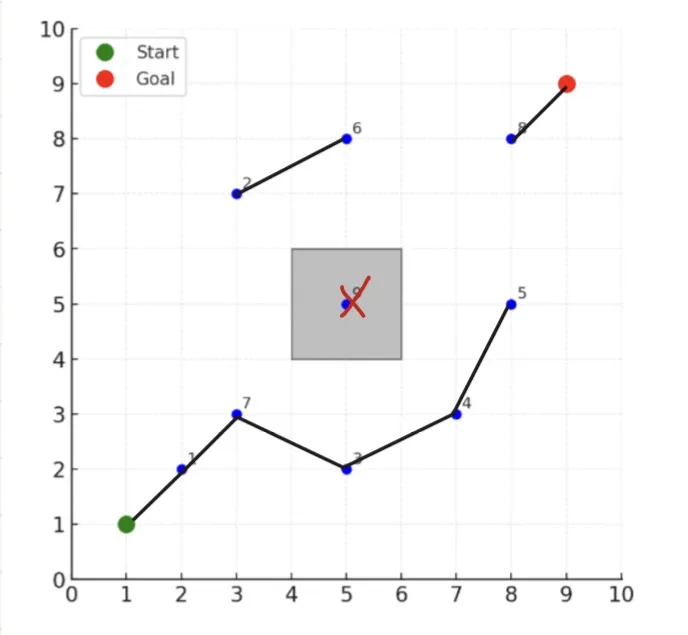
\includegraphics[width=0.6\textwidth]{roadmapimg.png}
    \caption{Constructed PRM roadmap showing valid samples (blue), start (green), goal (red), obstacle (gray), and edges connecting nodes within radius $r = 2.5$.}
    \label{fig:prm_roadmap}
\end{figure}


\subsubsection{Task 4: Search algorithm}

Running Dijkstra's algorithm from Start $(1,1)$:

The algorithm explores all nodes reachable from the start but cannot reach the goal because the graph is disconnected. The search terminates without finding a path.

\subsubsection{Task 5: Results and connectivity analysis}

\textbf{Path length:} No path exists.

\textbf{Number of nodes expanded:} Dijkstra's expands all nodes in the connected component containing the start: Start, $(2,2)$, $(3,3)$, $(3,7)$, $(5,2)$, $(5,8)$, $(7,3)$, $(8,5)$ = 8 nodes.

\textbf{Explanation:} The PRM fails to find a path because the roadmap is disconnected. The obstacle at $(4,4)$ to $(6,6)$ combined with the connection radius $r = 2.5$ creates a gap that prevents connectivity between the left and right sides of the workspace. The samples near the obstacle are too far apart to bridge this gap.

\textbf{Suggestions to improve connectivity:}
\begin{enumerate}
    \item \textbf{Increase connection radius:} Setting $r \geq 3.0$ would allow connections like $(5,8)$ to $(8,8)$ (distance = 3.0), bridging the gap around the obstacle
    \item \textbf{Add more samples:} Generating additional random samples, particularly in the region around the obstacle (e.g., near $(7,7)$ or $(3,5)$), would increase the likelihood of creating bridging connections
    \item \textbf{Use both approaches:} Combining more samples with a larger connection radius provides the most robust solution for ensuring connectivity
\end{enumerate}

\section{Problem 2: Randomly-Exploring Random Trees}





\end{document}